\documentclass[10pt, twoside]{article}
\usepackage{fancyhdr}
\usepackage{amsmath, amsthm, amssymb}
\usepackage[catalan]{babel}
\usepackage[titles]{tocloft}
\usepackage[utf8]{inputenc}
\usepackage[left=2.15cm, right=2.15cm, top=30mm, bottom=20mm]{geometry}
\usepackage{parskip}
\setlength{\parindent}{0pt} % Elimina la sangría de la primera línea de cada párrafo
\usepackage{titlesec}
\usepackage{bookmark}
\usepackage{multirow}
\usepackage{graphicx}
\usepackage{physics}
\usepackage{hyperref}
\usepackage{float}
\usepackage{caption}

\captionsetup{labelfont=bf}


\begin{document}

\begin{titlepage}
\centering
{\Large Fonaments d'Enginyeria Química \\ MO70399 \par}
\vspace{2cm}
{\Huge \textbf{Pràctica 2:} \par}
\vspace{1cm}
{\Huge \textbf{Balanç d'energia calorífica} \par}
\vspace{2cm}
{\Large Grup B \par}
\vspace{0.5cm}
{\Large Torn 2 \par}
\vspace{0.5cm}
{\normalsize Baldi Garcia, Isaac: 1667260 \\ Barbens Calzadilla, Carla: 1666167 \\ Belmonte Leiva, Marc: 1619451 \\ Bujones Umbert, Jun Shan: 1549086 \\ Franco Avilés, Eric: 1666739 \\ Gómez Rubio, Miquel: 1668850 \\ González Barea, Eric: 1672980 \\ Jacas García, Eira: 1666616 I NOMBRE DE PÀGINES AAAAAA\par}
\vspace{2cm}
{\Large Gener 2025 \par}
\vspace{2cm}

\includegraphics[width=0.4\textwidth]{Logo_UAB.png}


\end{titlepage}

\pagenumbering{gobble}
\renewcommand{\cftsecfont}{}
\renewcommand{\cftsecpagefont}{}
\renewcommand{\cftsecleader}{\cftdotfill{\cftdotsep}}
\renewcommand{\cftdotsep}{0.2}
\setlength{\cftbeforesecskip}{0.5em}
\setlength{\cftbeforesubsecskip}{0.5em}
\tableofcontents

\newpage
\pagenumbering{arabic}
\setcounter{page}{1}

\pagestyle{fancy}
\lhead{\textbf{Pràctica 2: Balanç d'energia calorífica}}
\rhead{\textbf{Fonaments d'Enginyeria Química}}

\begin{abstract}
En aquesta pràctica ens proposem estudiar els balaços d'energia calorífica aplicats tanc adiabàtic, en el qual no es produeix cap tipus d'intercanvi d'energia i/o matèria, i en concret de calor, amb l'entorn.  Per tal de demostrar experimentalment això, mesurarem la temperatura de l'aigua que flueix per dins del reactor en diferents temps, comparant-los amb la temperatura del tanc pulmó.
\end{abstract}

\section{Calibratge de la bomba i mesura del volum del tanc}
\subsection{Calibratge de la bomba}
Abans de començar amb la part experimental cal que, prèviament, calibrem la bomba, per tal de conèixer quins cabals es corresponen amb cada valor de rpm's de la bomba, i mesurem el volum del tanc. S'han obtingut els següents valors.
\begin{table}[h!]
    \centering
    \caption{Resultats obtinguts en el calibratge de la bomba.}
    \label{tab1}
    \begin{tabular}{|c|c|c|} % Estructura de columnas
    \hline
    Revolucions per minut (rpm) & Volum (mL) & Cabal (mL/min) \\ \hline
    90       & 625       & 208.33       \\ \hline
    110      & 760       & 253.33       \\ \hline
    130      & 910       & 303.33       \\ \hline
    \end{tabular}
\end{table}
 AQUÍ VA LA GRÀFICA DE LA CORBA DE CALIBRATGE
 
\subsection{Mesura del volum del tanc}
Els volums trobats trobats usant els dos mètodes proposats és\footnote{A l'annex s'explica en què consisteix cadascun dels dos mètodes.}:
\begin{itemize}
    \item \textbf{Mètode 1: }El volum obtingut ha estat $\Rightarrow$ $\boxed{V = 1595.00 \text{ mL}}$.
    \item \textbf{Mètode 2: }El volum obtingut ha estat $\Rightarrow$ $\boxed{V = 1637.98 \text{ mL}}$.
    \item \textbf{Volum promig: }El volum promig obtingut ha estat $\Rightarrow$ $\boxed{V = 1616.49 \text{ mL}}$.
\end{itemize}

\section{Resultats experimentals i discussió}

\subsection{Temperatures de sortida teòriques vs. experimentals}

\subsection{Evolució de temperatures teòriques vs. experimentals}

\subsection{Representació semilogarítmica de les temperatures experimentals}

\section{Conclusions}



\newpage
\appendix
{\Huge \textbf{Annexos}}

\section{Calibratge de la bomba d'entrada}
L'objectiu del calibratge és trobar per quins valors de rpm aconseguim treballar a uns cabals de 200 $\frac{\text{mL}}{\text{min}}$, 250 $\frac{\text{mL}}{\text{min}}$ i 300 $\frac{\text{mL}}{\text{min}}$. 

Per calibrar la bomba hem fet un seguit de mesures dels volums omplits per aquesta corresponents a una serie de valors de revolucions per minut (rpm) en un temps $t = 3$ min. Els valors obtinguts es poden veure a \ref{fig1}.

\begin{figure}[H]
    \centering
    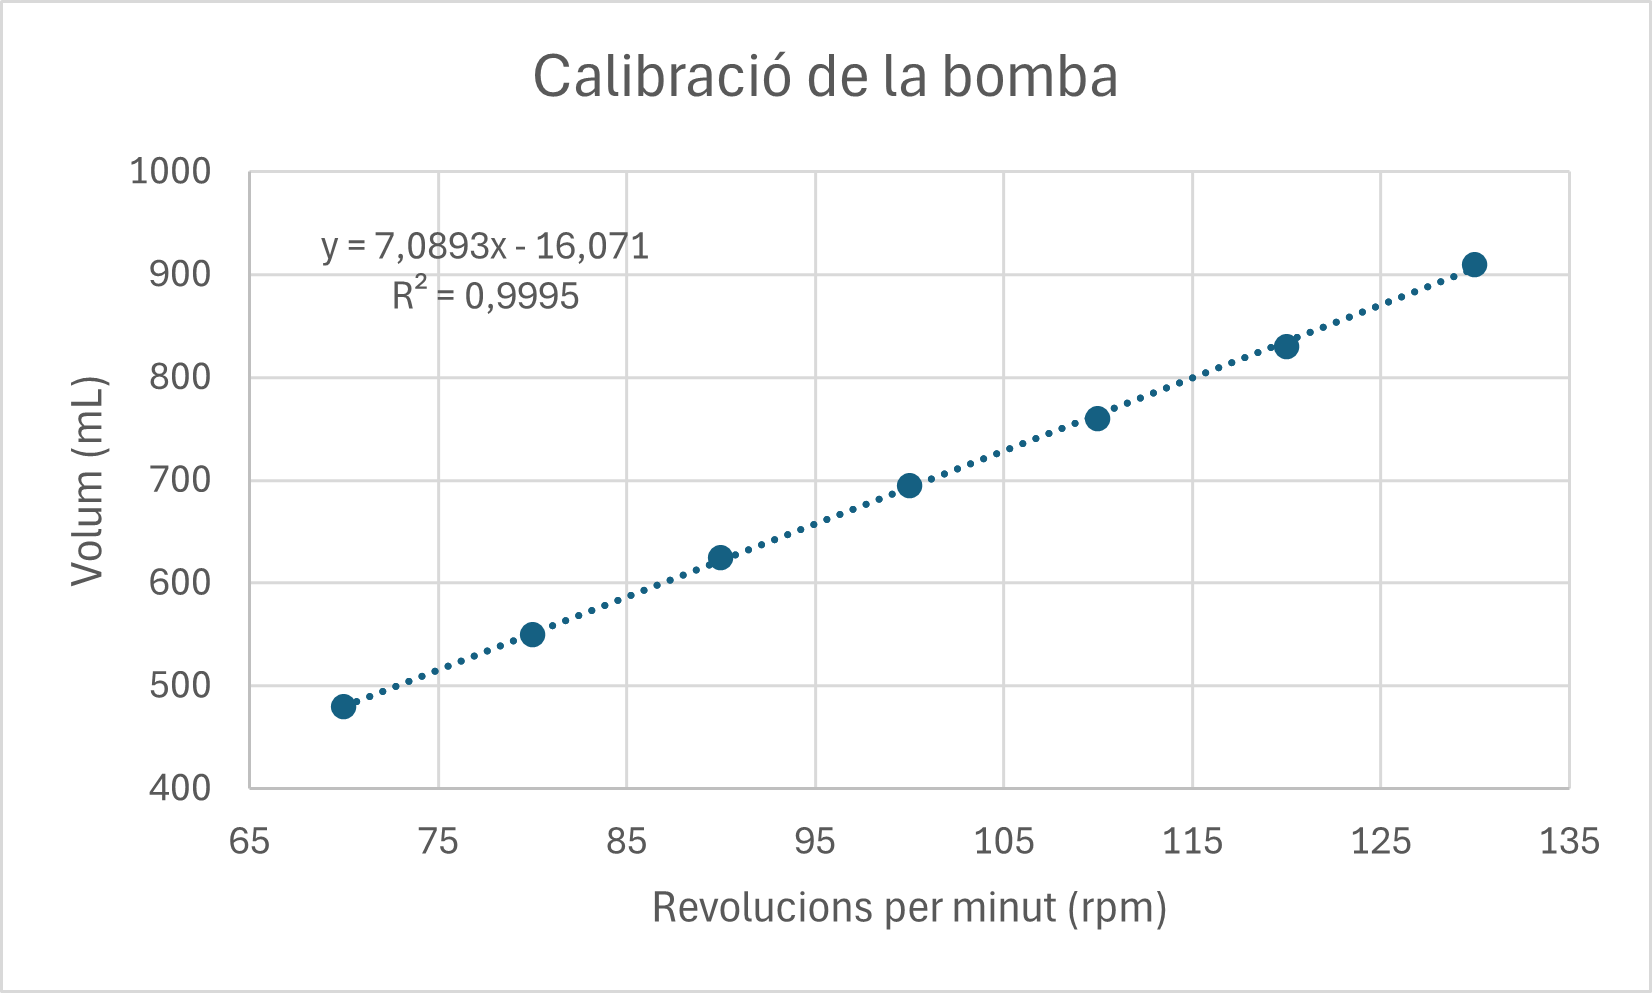
\includegraphics[width=0.7\linewidth]{calbomba.png}
    \caption{Resultats del calibratge de la bomba.}
    \label{fig1}
\end{figure}

L'equació obtinguda amb els nostres punts experimentals és $y=7.0893x-16.071$, amb una $R^2 = 0.9995$, valor que ens indica que les nostres mesures tenen una bona correlació lineal.

A partir d'aquí calculem els cabals corresponents a cada valor de revolucions per minut usant que

\begin{equation}
    Q_L = \frac{V}{t}
\end{equation}

on, de nou, $t=3$ min. Amb això fàcilment es pot determinar que els valors de rpm de la bomba necessaris per treballar a uns cabals de 200 $\frac{\text{mL}}{\text{min}}$, 250 $\frac{\text{mL}}{\text{min}}$ i 300 $\frac{\text{mL}}{\text{min}}$ són els donats a la taula \ref{tab1}.

\section{Mesura del volum del tanc}
Per tal de mesurar el volum del tanc amb el que hem treballat hem usat dos mètodes distints, tenint cura que les condicions de mesura eren exactament les condicions d'operació del tanc (agitador connectat al 10$\%$ de la seva potència màxima, sense xocar amb les parets del recipient i a una alçada fixada). Les dues metologies han estat:
\begin{enumerate}
    \item Omplir el tanc amb aigua i connectar la bomba de sortida. Quan la quantitat d'aigua que surt pel cabal de sortida és zero, mesurar tot el volum contingut al recipient (usant material volumètric del laboratori).
    \item Amb el tanc buit, connectar les bombes d'entrada i sortida. Mesurar el temps que triga a omplir-se el reactor. Amb aquest temps i el cabal (que és conegut, donat el valor de rpm de la bomba), es pot determinar $V$ usant
    \begin{equation}
        V = Q_L \cdot t
    \end{equation}
\end{enumerate}
El resultats obtinguts amb cada mètode es poden veure a la corresponent secció d'aquest informe.

\section{Presa de dades experimentals}
Per tal de trobar les temperatures  \textit{here goes blahblahblah}




\end{document}